\documentclass[12pt]{article}
%Fall 2022
% Some basic packages
\usepackage{standalone}[subpreambles=true]
\usepackage[utf8]{inputenc}
\usepackage[T1]{fontenc}
\usepackage{textcomp}
\usepackage[english]{babel}
\usepackage{url}
\usepackage{graphicx}
%\usepackage{quiver}
\usepackage{float}
\usepackage{enumitem}
\usepackage{lmodern}
\usepackage{comment}
\usepackage{hyperref}
\usepackage[usenames,svgnames,dvipsnames]{xcolor}
\usepackage[margin=1in]{geometry}
\usepackage{pdfpages}

\pdfminorversion=7

% Don't indent paragraphs, leave some space between them
\usepackage{parskip}

% Hide page number when page is empty
\usepackage{emptypage}
\usepackage{subcaption}
\usepackage{multicol}
\usepackage[b]{esvect}

% Math stuff
\usepackage{amsmath, amsfonts, mathtools, amsthm, amssymb}
\usepackage{bbm}
\usepackage{stmaryrd}
\allowdisplaybreaks

% Fancy script capitals
\usepackage{mathrsfs}
\usepackage{cancel}
% Bold math
\usepackage{bm}
% Some shortcuts
\newcommand{\rr}{\ensuremath{\mathbb{R}}}
\newcommand{\zz}{\ensuremath{\mathbb{Z}}}
\newcommand{\qq}{\ensuremath{\mathbb{Q}}}
\newcommand{\nn}{\ensuremath{\mathbb{N}}}
\newcommand{\ff}{\ensuremath{\mathbb{F}}}
\newcommand{\cc}{\ensuremath{\mathbb{C}}}
\newcommand{\ee}{\ensuremath{\mathbb{E}}}
\newcommand{\hh}{\ensuremath{\mathbb{H}}}
\renewcommand\O{\ensuremath{\emptyset}}
\newcommand{\norm}[1]{{\left\lVert{#1}\right\rVert}}
\newcommand{\dbracket}[1]{{\left\llbracket{#1}\right\rrbracket}}
\newcommand{\ve}[1]{{\bm{#1}}}
\newcommand\allbold[1]{{\boldmath\textbf{#1}}}
\DeclareMathOperator{\lcm}{lcm}
\DeclareMathOperator{\im}{im}
\DeclareMathOperator{\coim}{coim}
\DeclareMathOperator{\dom}{dom}
\DeclareMathOperator{\tr}{tr}
\DeclareMathOperator{\rank}{rank}
\DeclareMathOperator*{\var}{Var}
\DeclareMathOperator*{\ev}{E}
\DeclareMathOperator{\dg}{deg}
\DeclareMathOperator{\aff}{aff}
\DeclareMathOperator{\conv}{conv}
\DeclareMathOperator{\inte}{int}
\DeclareMathOperator*{\argmin}{argmin}
\DeclareMathOperator*{\argmax}{argmax}
\DeclareMathOperator{\graph}{graph}
\DeclareMathOperator{\sgn}{sgn}
\DeclareMathOperator*{\Rep}{Rep}
\DeclareMathOperator{\Proj}{Proj}
\DeclareMathOperator{\mat}{mat}
\DeclareMathOperator{\diag}{diag}
\DeclareMathOperator{\aut}{Aut}
\DeclareMathOperator{\gal}{Gal}
\DeclareMathOperator{\inn}{Inn}
\DeclareMathOperator{\edm}{End}
\DeclareMathOperator{\Hom}{Hom}
\DeclareMathOperator{\ext}{Ext}
\DeclareMathOperator{\tor}{Tor}
\DeclareMathOperator{\Span}{Span}
\DeclareMathOperator{\Stab}{Stab}
\DeclareMathOperator{\cont}{cont}
\DeclareMathOperator{\Ann}{Ann}
\DeclareMathOperator{\Div}{div}
\DeclareMathOperator{\curl}{curl}
\DeclareMathOperator{\nat}{Nat}
\DeclareMathOperator{\gr}{Gr}
\DeclareMathOperator{\vect}{Vect}
\DeclareMathOperator{\id}{id}
\DeclareMathOperator{\Mod}{Mod}
\DeclareMathOperator{\sign}{sign}
\DeclareMathOperator{\Surf}{Surf}
\DeclareMathOperator{\fcone}{fcone}
\DeclareMathOperator{\Rot}{Rot}
\DeclareMathOperator{\grad}{grad}
\DeclareMathOperator{\atan2}{atan2}
\DeclareMathOperator{\Ric}{Ric}
\let\vec\relax
\DeclareMathOperator{\vec}{vec}
\let\Re\relax
\DeclareMathOperator{\Re}{Re}
\let\Im\relax
\DeclareMathOperator{\Im}{Im}
% Put x \to \infty below \lim
\let\svlim\lim\def\lim{\svlim\limits}

%wide hat
\usepackage{scalerel,stackengine}
\stackMath
\newcommand*\wh[1]{%
\savestack{\tmpbox}{\stretchto{%
  \scaleto{%
    \scalerel*[\widthof{\ensuremath{#1}}]{\kern-.6pt\bigwedge\kern-.6pt}%
    {\rule[-\textheight/2]{1ex}{\textheight}}%WIDTH-LIMITED BIG WEDGE
  }{\textheight}% 
}{0.5ex}}%
\stackon[1pt]{#1}{\tmpbox}%
}
\parskip 1ex

%Make implies and impliedby shorter
\let\implies\Rightarrow
\let\impliedby\Leftarrow
\let\iff\Leftrightarrow
\let\epsilon\varepsilon

% Add \contra symbol to denote contradiction
\usepackage{stmaryrd} % for \lightning
\newcommand\contra{\scalebox{1.5}{$\lightning$}}

% \let\phi\varphi

% Command for short corrections
% Usage: 1+1=\correct{3}{2}

\definecolor{correct}{HTML}{009900}
\newcommand\correct[2]{\ensuremath{\:}{\color{red}{#1}}\ensuremath{\to }{\color{correct}{#2}}\ensuremath{\:}}
\newcommand\green[1]{{\color{correct}{#1}}}

% horizontal rule
\newcommand\hr{
    \noindent\rule[0.5ex]{\linewidth}{0.5pt}
}

% hide parts
\newcommand\hide[1]{}

% si unitx
\usepackage{siunitx}
\sisetup{locale = FR}

%allows pmatrix to stretch
\makeatletter
\renewcommand*\env@matrix[1][\arraystretch]{%
  \edef\arraystretch{#1}%
  \hskip -\arraycolsep
  \let\@ifnextchar\new@ifnextchar
  \array{*\c@MaxMatrixCols c}}
\makeatother

\renewcommand{\arraystretch}{0.8}

\renewcommand{\baselinestretch}{1.5}

\usepackage{graphics}
\usepackage{epstopdf}

\RequirePackage{hyperref}
%%
%% Add support for color in order to color the hyperlinks.
%% 
\hypersetup{
  colorlinks = true,
  urlcolor = blue,
  citecolor = blue
}
%%fakesection Links
\hypersetup{
    colorlinks,
    linkcolor={red!50!black},
    citecolor={green!50!black},
    urlcolor={blue!80!black}
}
%customization of cleveref
\RequirePackage[capitalize,nameinlink]{cleveref}[0.19]

% Per SIAM Style Manual, "section" should be lowercase
\crefname{section}{section}{sections}
\crefname{subsection}{subsection}{subsections}
\Crefname{section}{Section}{Sections}
\Crefname{subsection}{Subsection}{Subsections}

% Per SIAM Style Manual, "Figure" should be spelled out in references
\Crefname{figure}{Figure}{Figures}

% Per SIAM Style Manual, don't say equation in front on an equation.
\crefformat{equation}{\textup{#2(#1)#3}}
\crefrangeformat{equation}{\textup{#3(#1)#4--#5(#2)#6}}
\crefmultiformat{equation}{\textup{#2(#1)#3}}{ and \textup{#2(#1)#3}}
{, \textup{#2(#1)#3}}{, and \textup{#2(#1)#3}}
\crefrangemultiformat{equation}{\textup{#3(#1)#4--#5(#2)#6}}%
{ and \textup{#3(#1)#4--#5(#2)#6}}{, \textup{#3(#1)#4--#5(#2)#6}}{, and \textup{#3(#1)#4--#5(#2)#6}}

% But spell it out at the beginning of a sentence.
\Crefformat{equation}{#2Equation~\textup{(#1)}#3}
\Crefrangeformat{equation}{Equations~\textup{#3(#1)#4--#5(#2)#6}}
\Crefmultiformat{equation}{Equations~\textup{#2(#1)#3}}{ and \textup{#2(#1)#3}}
{, \textup{#2(#1)#3}}{, and \textup{#2(#1)#3}}
\Crefrangemultiformat{equation}{Equations~\textup{#3(#1)#4--#5(#2)#6}}%
{ and \textup{#3(#1)#4--#5(#2)#6}}{, \textup{#3(#1)#4--#5(#2)#6}}{, and \textup{#3(#1)#4--#5(#2)#6}}

% Make number non-italic in any environment.
\crefdefaultlabelformat{#2\textup{#1}#3}

% Environments
\makeatother
% For box around Definition, Theorem, \ldots
%%fakesection Theorems
\usepackage{thmtools}
\usepackage[framemethod=TikZ]{mdframed}

\theoremstyle{definition}
\mdfdefinestyle{mdbluebox}{%
	roundcorner = 10pt,
	linewidth=1pt,
	skipabove=12pt,
	innerbottommargin=9pt,
	skipbelow=2pt,
	nobreak=true,
	linecolor=blue,
	backgroundcolor=TealBlue!5,
}
\declaretheoremstyle[
	headfont=\sffamily\bfseries\color{MidnightBlue},
	mdframed={style=mdbluebox},
	headpunct={\\[3pt]},
	postheadspace={0pt}
]{thmbluebox}

\mdfdefinestyle{mdredbox}{%
	linewidth=0.5pt,
	skipabove=12pt,
	frametitleaboveskip=5pt,
	frametitlebelowskip=0pt,
	skipbelow=2pt,
	frametitlefont=\bfseries,
	innertopmargin=4pt,
	innerbottommargin=8pt,
	nobreak=false,
	linecolor=RawSienna,
	backgroundcolor=Salmon!5,
}
\declaretheoremstyle[
	headfont=\bfseries\color{RawSienna},
	mdframed={style=mdredbox},
	headpunct={\\[3pt]},
	postheadspace={0pt},
]{thmredbox}

\declaretheorem[%
style=thmbluebox,name=Theorem,numberwithin=section]{thm}
\declaretheorem[style=thmbluebox,name=Lemma,sibling=thm]{lem}
\declaretheorem[style=thmbluebox,name=Proposition,sibling=thm]{prop}
\declaretheorem[style=thmbluebox,name=Corollary,sibling=thm]{coro}
\declaretheorem[style=thmredbox,name=Example,sibling=thm]{eg}

\mdfdefinestyle{mdgreenbox}{%
	roundcorner = 10pt,
	linewidth=1pt,
	skipabove=12pt,
	innerbottommargin=9pt,
	skipbelow=2pt,
	nobreak=true,
	linecolor=ForestGreen,
	backgroundcolor=ForestGreen!5,
}

\declaretheoremstyle[
	headfont=\bfseries\sffamily\color{ForestGreen!70!black},
	bodyfont=\normalfont,
	spaceabove=2pt,
	spacebelow=1pt,
	mdframed={style=mdgreenbox},
	headpunct={ --- },
]{thmgreenbox}

\declaretheorem[style=thmgreenbox,name=Definition,sibling=thm]{defn}

\mdfdefinestyle{mdgreenboxsq}{%
	linewidth=1pt,
	skipabove=12pt,
	innerbottommargin=9pt,
	skipbelow=2pt,
	nobreak=true,
	linecolor=ForestGreen,
	backgroundcolor=ForestGreen!5,
}
\declaretheoremstyle[
	headfont=\bfseries\sffamily\color{ForestGreen!70!black},
	bodyfont=\normalfont,
	spaceabove=2pt,
	spacebelow=1pt,
	mdframed={style=mdgreenboxsq},
	headpunct={},
]{thmgreenboxsq}
\declaretheoremstyle[
	headfont=\bfseries\sffamily\color{ForestGreen!70!black},
	bodyfont=\normalfont,
	spaceabove=2pt,
	spacebelow=1pt,
	mdframed={style=mdgreenboxsq},
	headpunct={},
]{thmgreenboxsq*}

\mdfdefinestyle{mdblackbox}{%
	skipabove=8pt,
	linewidth=3pt,
	rightline=false,
	leftline=true,
	topline=false,
	bottomline=false,
	linecolor=black,
	backgroundcolor=RedViolet!5!gray!5,
}
\declaretheoremstyle[
	headfont=\bfseries,
	bodyfont=\normalfont\small,
	spaceabove=0pt,
	spacebelow=0pt,
	mdframed={style=mdblackbox}
]{thmblackbox}

\theoremstyle{plain}
\declaretheorem[name=Question,sibling=thm,style=thmblackbox]{ques}
\declaretheorem[name=Remark,sibling=thm,style=thmgreenboxsq]{remark}
\declaretheorem[name=Remark,sibling=thm,style=thmgreenboxsq*]{remark*}
\newtheorem{ass}[thm]{Assumptions}

\theoremstyle{definition}
\newtheorem*{problem}{Problem}
\newtheorem{claim}[thm]{Claim}
\theoremstyle{remark}
\newtheorem*{case}{Case}
\newtheorem*{notation}{Notation}
\newtheorem*{note}{Note}
\newtheorem*{motivation}{Motivation}
\newtheorem*{intuition}{Intuition}
\newtheorem*{conjecture}{Conjecture}

% Make section starts with 1 for report type
%\renewcommand\thesection{\arabic{section}}

% End example and intermezzo environments with a small diamond (just like proof
% environments end with a small square)
\usepackage{etoolbox}
\AtEndEnvironment{vb}{\null\hfill$\diamond$}%
\AtEndEnvironment{intermezzo}{\null\hfill$\diamond$}%
% \AtEndEnvironment{opmerking}{\null\hfill$\diamond$}%

% Fix some spacing
% http://tex.stackexchange.com/questions/22119/how-can-i-change-the-spacing-before-theorems-with-amsthm
\makeatletter
\def\thm@space@setup{%
  \thm@preskip=\parskip \thm@postskip=0pt
}

% Fix some stuff
% %http://tex.stackexchange.com/questions/76273/multiple-pdfs-with-page-group-included-in-a-single-page-warning
\pdfsuppresswarningpagegroup=1


% My name
\author{Jaden Wang}


%include Matlab code
\usepackage{sectsty}
\usepackage{listings}
\usepackage{color}
\usepackage{alltt}
\definecolor{dkgreen}{rgb}{0,0.6,0}
\definecolor{gray}{rgb}{0.5,0.5,0.5}
\definecolor{mauve}{rgb}{0.58,0,0.82}

\lstset{frame=tb,
  language=Matlab,
  aboveskip=3mm,
  belowskip=3mm,
  showstringspaces=false,
  columns=flexible,
  basicstyle={\small\ttfamily},
  numbers=none,
  numberstyle=\tiny\color{gray},
  keywordstyle=\color{blue},
  commentstyle=\color{dkgreen},
  stringstyle=\color{mauve},
  breaklines=true,
  breakatwhitespace=true,
  tabsize=3
}
\begin{document}
\centerline {\textsf{\textbf{\LARGE{Homework 2}}}}
\centerline {Jaden Wang}
\vspace{.15in}

\begin{problem}[1]
Since $ Dg(x,y) = \begin{bmatrix} 4x^3-3x^2\\2y \end{bmatrix}$, it equals zero exactly when $ y=0$ and  $ x=0$ or  $ \frac{4}{3}$. Strong normality is satisfied for all other points. This this case, the Lagrangian is
\begin{align*}
	\mathscr{L}((x,y),1,\lambda) = x + \lambda(y^2+x^{4} - x^3) .
\end{align*}
The first-order conditions require that
\begin{align*}
	\mathscr{L}_x &= 1+4\lambda x^3-3\lambda x^2 =0\\
	\mathscr{L}_y &= 2\lambda y =0\\
	\mathscr{L}_\lambda &= y^2+x^{4}-x^3=0 
\end{align*}
which forces $ y=0$,  $ x=1$, and thus  $ \lambda = -1$. Thus $ (1,0) \in \inte \rr^2$ is a candidate local minimizer.  Since $ g'(1,0) = \begin{bmatrix} 1\\0 \end{bmatrix} $, the null space is $ N = t \begin{bmatrix} 0\\1 \end{bmatrix} $. Since 
\begin{align*}
	\mathscr{L}_{(x,y) (x,y)} = \begin{pmatrix} -12x^2+6x & 0\\0& -2 \end{pmatrix} 
\end{align*}
we see that for the basis vector of  $ N$,
\begin{align*}
	\begin{pmatrix} 0&1 \end{pmatrix} \begin{pmatrix} -6&0\\0&-2 \end{pmatrix} \begin{pmatrix} 0\\1 \end{pmatrix} = -2 <0 
\end{align*}
Thus $ (1,0)$ is not a local minimum. The only remaining possibilities are the abnormal cases $ (0,0)$ or $ (\frac{4}{3},0)$. The Lagrangian is
\begin{align*}
	\mathscr{L}((x,y),0,\lambda) &= \lambda(y^2+x^{4}-x^3) \\
	\mathscr{L}_x &= 4 \lambda x^3-3 \lambda x^2 =0 \\
	\mathscr{L}_y &= 0 \\
	\mathscr{L}_\lambda &= 0 
\end{align*}
which yields $ x=0$,  $ y=0$, and  $ \lambda$ can be anything nonzero. I claim that $ (0,0)$ is the global minimum. Suppose $ x<0$, then $ x^{4} >0$ and $ -x^3 >0$, thus $ y^2 + x^{4} - x^3 >0$, not satisfying the constraint. Thus $ f(x)$ is lower bounded by  $ x=0$, which is achieved by  $ (0,0)$.
\end{problem}

\begin{problem}[2]
For $ \mu=1$:
\begin{align*}
	\mathscr{L}(x,1,\lambda,\nu) = x_1^2 - x_2 + \lambda_1(x_1^2+x_2^2-1) &+ \lambda_2(x_2-2)+ \nu(x_1^3+x_2-1) \\
	\mathscr{L}_x= \begin{pmatrix} x_1(2+2 \lambda_1 + 3 \nu x_1)\\ 2\lambda_1 x_2+ \lambda_2 + \nu-1 \end{pmatrix} &= \begin{pmatrix} 0\\0 \end{pmatrix}  \\
	\lambda_1 (x_1^2+x_2^2 -1 ) &= 0 \\
	\lambda_2 (x_2 -2) &= 0 \\
	\lambda_1 , \lambda_2  &\geq 0\\
	x_1^3+x_2-1 &= 0 \\
	x_1^2+x_2^2 -1 &\leq 0\\
	x_2 -2	& \leq 0
\end{align*}
Since if $ x_2^*=2$, $ x_1^2+(x_2^*)^2-1 = x_1^2 + 3 >0$ not primal feasible, so it must be that $ \lambda_2^* = 0$. The solutions that satisfy the system of equations and inequality constraints above are $ x_1=0$, $ x_2 =1$, $\lambda_2=0$, and $ \nu=1-2 \lambda_1$; $ x_1= 0.544, x_2= 0.839, \lambda_1 = 4.92, \lambda_2 = 0,$ and $ \nu= -7.26$.

We see that only $ \lambda_1$ is active, so the Jacobian to test normality is
\begin{align*}
	\nabla \begin{pmatrix} x_1^2+x_2^2\\x_1^3+x_2 \end{pmatrix}  &= \begin{pmatrix} 2x_1&2x_2\\3x_1^2&1 \end{pmatrix}
\end{align*}
Since $ \ell=2$, the only time this matrix is not rank 2 is when $ x_1 =0$. This means that our solution $ (0,1)$ is abnormal, but $ (0.544,0.839)$ is strongly normal.

\begin{align*}
	\mathscr{L}_{x x} &= \begin{pmatrix} 6\nu x_1+2\lambda_1+2&0\\0&2\lambda_1 \end{pmatrix} = \begin{pmatrix} -11.86&0\\0&9.84 \end{pmatrix}  \\
\end{align*}
is a local saddle point.

When $ \mu=0$,
\begin{align*}
	\mathscr{L}(x,0,\lambda,\nu) = \lambda_1(x_1^2+x_2^2-1) &+ \lambda_2(x_2-2)+ \nu(x_1^3+x_2-1) \\
	\mathscr{L}_x= \begin{pmatrix} x_1(2 \lambda_1 + 3 \nu x_1)\\ 2\lambda_1 x_2+ \lambda_2 + \nu \end{pmatrix} &= \begin{pmatrix} 0\\0 \end{pmatrix}  \\
	\lambda_1 (x_1^2+x_2^2 -1 ) &= 0 \\
	\lambda_2 (x_2 -2) &= 0 \\
	\lambda_1 , \lambda_2  &\geq 0\\
	x_1^3+x_2-1 &= 0 \\
	x_1^2+x_2^2 -1 &\leq 0\\
	x_2 -2	& \leq 0
\end{align*}
and we get the same solution as the case when $ \mu=1$.

Since this is the only candidate, $ (0,1)$ is the minimizer we seek, the minimum is $ f(0,1)=-1$.
\end{problem}
\begin{problem}[3]
Since maximizing $ x_1$ is the same as minimizing $ -x_1$, we have $ f(x_1,x_2) = -x_1$  For all other points, assume $ \mu=1$:
\begin{align*}
	\mathscr{L}(x_1,x_2,1,\lambda_1,\lambda_2) &= -x_1 + \lambda_1(x_2-(1-x_1)^3)-\lambda_2 x_2\\
	\mathscr{L}_x = \begin{pmatrix} -1+3\lambda_1(1-x_1)^2\\ \lambda_1-\lambda_2 \end{pmatrix} &=0 \\
	\lambda_1(x_2-(1-x_1)^3) &= 0 \\
	-\lambda_2 x_2 &= 0 \\
	\lambda_1,\lambda_2 &\geq 0\\
	x_2-(1-x_1)^3 &\leq 0\\
	-x_2 &\leq 0 
\end{align*}
We see that $ \lambda_2 \neq 0$ since otherwise $ \lambda_1 =0$ and we have $ -1 =0$. It must be that  $ x_2 = 0$ and thus $ -(1-x_1)^3=0$ which forces $ x_1 = 1$, but this violates the first equation, so there is no solution.

Now for $ \mu=0$,
\begin{align*}
	\mathscr{L}(x_1,x_2,0,\lambda_1,\lambda_2) &= \lambda_1(x_2-(1-x_1)^3)-\lambda_2 x_2\\
	\mathscr{L}_x = \begin{pmatrix} 3\lambda_1(1-x_1)^2\\ \lambda_1-\lambda_2 \end{pmatrix} &=0 \\
	\lambda_1(x_2-(1-x_1)^3) &= 0 \\
	-\lambda_2 x_2 &= 0 \\
	\lambda_1,\lambda_2 &\geq 0\\
	x_2-(1-x_1)^3 &\leq 0\\
	-x_2 &\leq 0 
\end{align*}
The solution is $ (1,0)$ with both constraints active. We have $ g(x_1,x_2) = \begin{pmatrix} x_2 - (1-x_1)^3\\-x_2 \end{pmatrix} $.
\begin{align*}
	g'(x_1,x_2) = \begin{pmatrix} 3(1-x_1)^2&1\\0&-1 \end{pmatrix} 
\end{align*}
Thus the point is abnormal iff $ x_1=1$. So $ (1,0)$ is abnormal! Thus the maximum of  $ x_1$ is achieved at 1.
~\begin{figure}[H]
	\centering
	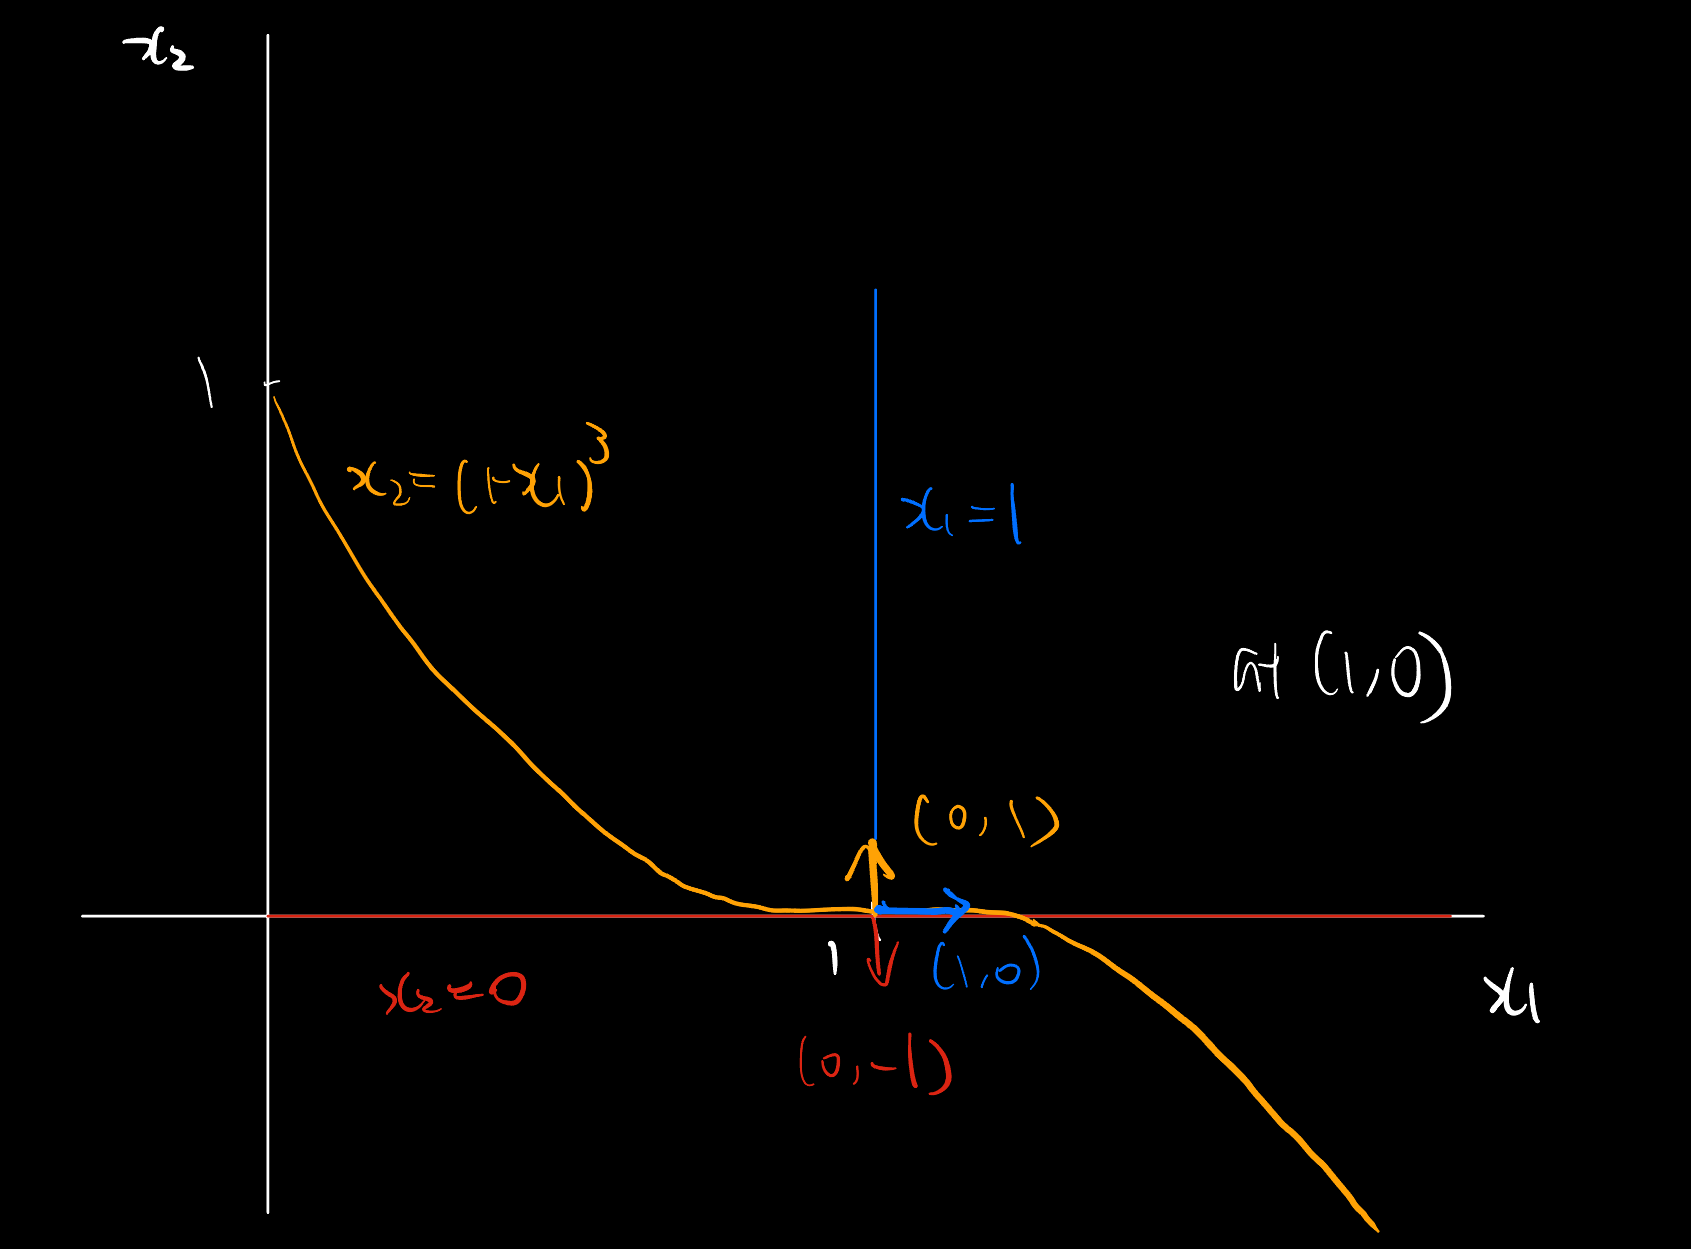
\includegraphics[width=0.7\textwidth]{./figures/gradient.png}
	\caption{We see that at $ (0,1)$ the gradients of two active constraints are parallel.}
\end{figure}
\end{problem}
\begin{problem}[4]
For $ \mu=1$, we have
\begin{align*}
	\mathscr{L}(x,1,\lambda) = -5x_1-x_2 +\lambda_1(-x_1) + \lambda_2 & (3x_1+x_2-11)+ \lambda_3(x_1-2x_2-2) \\
	\mathscr{L}_x = \begin{pmatrix}  -5-\lambda_1+3\lambda_2+\lambda_3\\ -1+\lambda_2-2\lambda_3 \end{pmatrix}  &= \begin{pmatrix} 0\\0 \end{pmatrix}  \\
	\lambda_1(-x_1) &= 0 \\
	\lambda_2(3x_1+x_2-11) &= 0 \\
	\lambda_3(x_1-2x_2-2) &= 0 \\
	\lambda_1,\lambda_2,\lambda_3 &\geq 0\\
	-x_1 &\leq 0\\
	3x_1+x_2-11 &\leq 0\\
	x_1-2x_2-2 & \leq 0
\end{align*}
The only solution is $ x_1= \frac{24}{7}$, $ x_2 = \frac{5}{7}$, $ \lambda_1 = 0$, $ \lambda_2=\frac{11}{7}$, and $ \lambda_3 = \frac{2}{7}$.

Since $ \lambda_1=0$, the Jacobian to test normality is
We compute
\begin{align*}
	\nabla \begin{pmatrix} 3x_1+x_2-11\\x_1-2x_2-2 \end{pmatrix}  &= \begin{pmatrix} 3&1\\1&-2 \end{pmatrix}  
\end{align*}
which has rank $ 2$, same as the dimension of its image. Thus the solution is strongly normal.

\begin{align*}
	\mathscr{L}_{x x} = \begin{pmatrix} 0&0\\0&0 \end{pmatrix} 
\end{align*}

For $ \mu=0$, we have
\begin{align*}
	\mathscr{L}(x,0,\lambda) = \lambda_1(-x_1) + \lambda_2 & (3x_1+x_2-11)+ \lambda_3(x_1-2x_2-2) \\
	\mathscr{L}_x = \begin{pmatrix}  -\lambda_1+3\lambda_2+\lambda_3\\ \lambda_2-2\lambda_3 \end{pmatrix}  &= \begin{pmatrix} 0\\0 \end{pmatrix}  \\
	\lambda_1(-x_1) &= 0 \\
	\lambda_2(3x_1+x_2-11) &= 0 \\
	\lambda_3(x_1-2x_2-2) &= 0 \\
	\lambda_1,\lambda_2,\lambda_3 &\geq 0\\
	-x_1 &\leq 0\\
	3x_1+x_2-11 &\leq 0\\
	x_1-2x_2-2 & \leq 0
\end{align*}
which has no solution with one of multipliers nonzero.
~\begin{figure}[H]
	\centering
	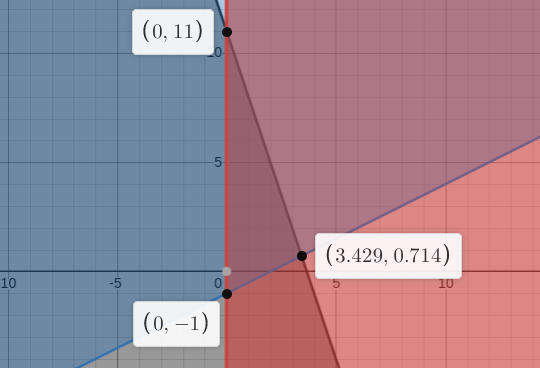
\includegraphics[width=0.6\textwidth]{./figures/feasible_region}
	\caption{The feasible region is the triangle formed by the three points. We see that the minimizer is at a vertex of the triangle.}
	\label{fig:feasible_region}
\end{figure}
The minimum is therefore $ -5 \cdot \frac{24}{7}-\frac{5}{7} = -\frac{125}{ 7}$.

\begin{lstlisting}
%%%%%%%%%%%%%%%%%%%%%%%%%%%%%%%%%%%%%%%%%%%%%%%%%%%%%%%%%%%%%%%%%%%%%%%%%%
%Problem 4
function [c,ceq] = constraints4(x)
x1=x(1);
x2=x(2);
c=[-x1;3*x1+x2-11;x1-2*x2-2];
ceq = [];
%%%%%%%%%%%%%%%%%%%%%%%%%%%%%%%%%%%%%%%%%%%%%%%%%%%%%%%%%%%%%%%%%%%%%%%%%%
f=@(x) -5*x(1)-x(2);
A = [];
b = [];
Aeq = [];
beq = [];
lb = [];
ub = [];
nonlcon=@constraints4;
x0=[1;0];
x=fmincon(f,x0,A,b,Aeq,beq,lb,ub,nonlcon)
fx = f(x)
%%%%%%%%%%%%%%%%%%%%%%%%%%%%%%%%%%%%%%%%%%%%%%%%%%%%%%%%%%%%%%%%%%%%%%%%%%
\end{lstlisting}
The output is a match!
\end{problem}

\begin{problem}[5]
\begin{enumerate}[label=(\arabic*)]
	\item \begin{align*}
	\min\quad & \begin{pmatrix} 400&360&550&470&600&500 \end{pmatrix} \begin{pmatrix} x_1&x_2&x_3&x_4&x_5&x_6 \end{pmatrix}^{T}  \\
	\text{subject to } \quad & \begin{pmatrix} 1&1&0&0&0&0\\0&0&1&1&0&0\\0&0&0&0&1&1\\1&0&1&0&1&0\\0&1&0&1&0&1 \end{pmatrix} \begin{pmatrix} x_1&x_2&x_3&x_4&x_5&x_6 \end{pmatrix}^{T}  = \begin{pmatrix} 200\\360\\340\\500\\400 \end{pmatrix} 
\end{align*}
\item 
\begin{lstlisting}
%%%%%%%%%%%%%%%%%%%%%%%%%%%%%%%%%%%%%%%%%%%%%%%%%%%%%%%%%%%%%%%%%%%%%%%%%%
%Problem 5
f=[400;360;550;470;600;500];
A = [];
b = [];
Aeq = [1 1 0 0 0 0;0 0 1 1 0 0; 0 0 0 0 1 1; 1 0 1 0 1 0; 0 1 0 1 0 1];
beq = [200;360;340;500;400];
lb = [0;0;0;0;0;0];
ub = [500;400;500;400;500;400];
x=linprog(f,A,b,Aeq,beq,lb,ub);
fx=f'*x
%%%%%%%%%%%%%%%%%%%%%%%%%%%%%%%%%%%%%%%%%%%%%%%%%%%%%%%%%%%%%%%%%%%%%%%%%%
\end{lstlisting}

The minimum cost schedule is $ \begin{pmatrix} 200&0&300&60&0&340 \end{pmatrix}^T $ and the minimum cost is $ 443200$ dollars.

\end{enumerate}
\end{problem}

\begin{problem}[6]
\begin{enumerate}[label=(\arabic*)]
	\item 
\begin{align*}
	\mathscr{L}= V \sin \gamma + \lambda_1 (T(V)\cos( \alpha+ \epsilon)- D(V, \alpha) - mg \sin \gamma) + \lambda_2 (T(V) \sin ( \alpha + \epsilon)+ L(V, \alpha)- mg \cos \gamma)
\end{align*}
So the first-order necessary conditions are
\begin{align*}
	\mathscr{L}_V &= \sin \gamma + \lambda_1 (T'(V) \cos ( \alpha+ \epsilon)-D_V(V, \alpha)) + \lambda_2(T'(V) \sin ( \alpha + \epsilon)+L_V(V, \alpha)) =0 \\
	&= \sin \gamma + (\lambda_1\cos ( \alpha + 0.0349)+ \lambda_2 \sin ( \alpha+ 0.0349)) ( -0.04312+2 \cdot 0.008392V)\\ 
	& \quad -2\lambda_1V(0.07351-0.08617 \alpha+1.996 \alpha^2) +  2\lambda_2 V (0.1667+6.231 \alpha - 21.65 [ \max (0, \alpha - 0.2094)]^2)\\
	\mathscr{L}_{ \alpha} &= -\lambda_1 (T(V) \sin ( \alpha+ \epsilon) - V^2(-0.08617+2 \cdot 1.996 \alpha +6.231-2 \cdot  21.65[(\alpha - 0.2094) \text{ or } 0]) )\\
	\mathscr{L}_{ \gamma} &= (V-mg) \cos \gamma + mg \sin \gamma \\
	0&=T(V) \cos( \alpha + \epsilon)-D(V, \alpha) - mg \sin \gamma \\
0&=T(V) \sin ( \alpha+ \epsilon) + L(V, \alpha)-mg \cos \gamma 
\end{align*}

\item
\begin{lstlisting}
%%%%%%%%%%%%%%%%%%%%%%%%%%%%%%%%%%%%%%%%%%%%%%%%%%%%%%%%%%%%%%%%%%%%%%%%%%
%Problem 6b
function [c,ceq] = constraints6(x)
T=@(V) 0.2476-0.04312*V+0.008392*V^2;
D=@(V,a) V^2*(0.07351-0.08617*a+1.996*a^2);
L=@(V,a) V^2*(0.1667+6.231*a-21.65*(max([0 a-0.2094])^2));
e=0.0349;
w=180000;
c=[];
V=x(1);
a=x(2);
gamma=x(3);
ceq = [T(V)*cos(a+e)-D(V,a)-w*sin(gamma);T(V)*sin(a+e)+L(V,a)-w*cos(gamma)];
%%%%%%%%%%%%%%%%%%%%%%%%%%%%%%%%%%%%%%%%%%%%%%%%%%%%%%%%%%%%%%%%%%%%%%%%%%
g=32.17;
W=180000;
l=2*W/(0.002203*1560*g);
f=@(x) -x(1)*sin(x(3)); %maximize is the same as minimize the negative
A = [];
b = [];
Aeq = [];
beq = [];
lb = [1,0.1,0.1];
ub = [2,0.2,0.2];
nonlcon=@constraints6;
x0=[342/sqrt(g*l);6.39/180*pi;6.31/180*pi];
[x,fval,exitflag,output,lambda,grad,hessian]=fmincon(f,x0,A,b,Aeq,beq,lb,ub,nonlcon)
fval
%%%%%%%%%%%%%%%%%%%%%%%%%%%%%%%%%%%%%%%%%%%%%%%%%%%%%%%%%%%%%%%%%%%%%%%%%%
\end{lstlisting}
I cannot get the correct values after hours of debugging.

\item I do not have the lambdas from b so I cannot check if it is zero.

\end{enumerate}
\end{problem}
\end{document}
